\documentclass[border=5pt]{standalone}
\usepackage{tikz}
\usepackage{xcolor}

\definecolor{danger}{RGB}{220,53,69}
\definecolor{warning}{RGB}{255,193,7}
\definecolor{secondary}{RGB}{108,117,125}
\definecolor{success}{RGB}{40,167,69}
\definecolor{info}{RGB}{23,162,184}

\begin{document}
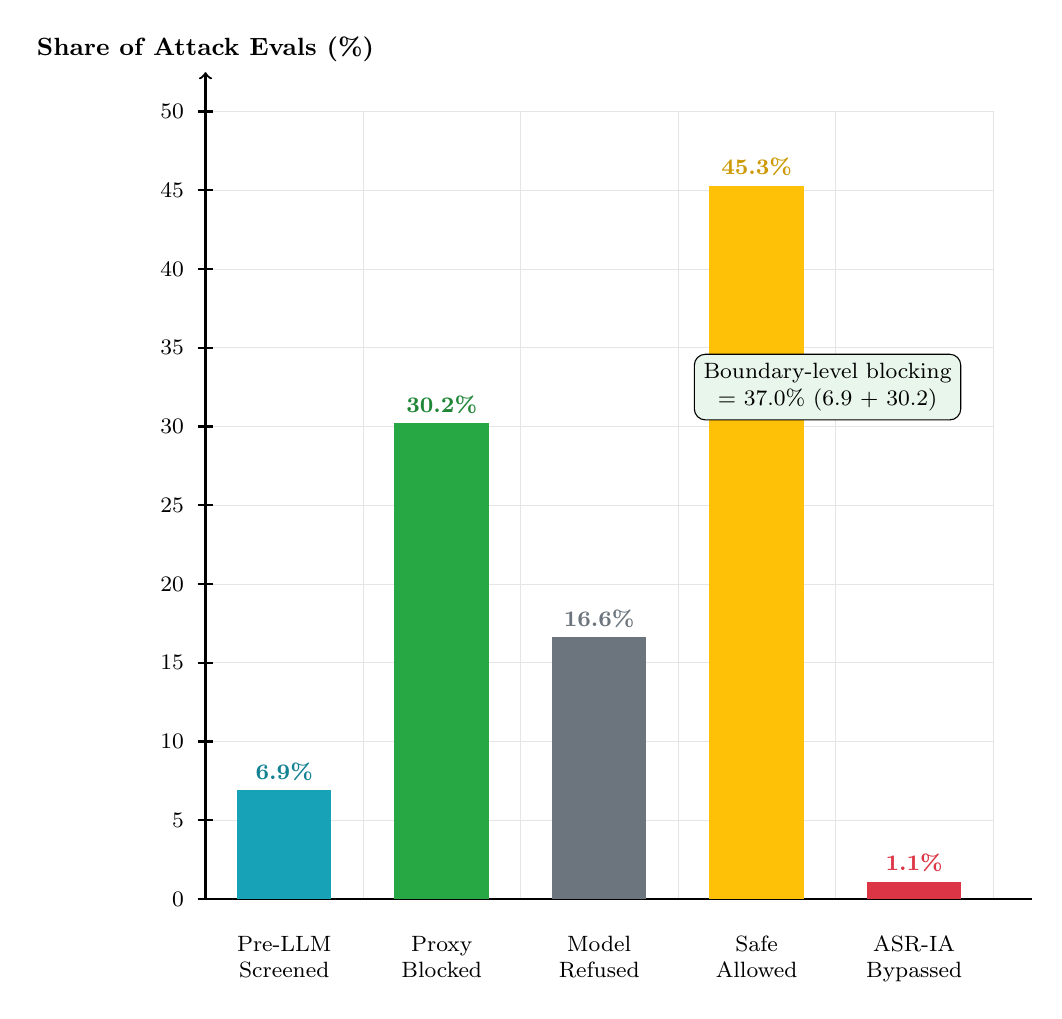
\begin{tikzpicture}[scale=1]
  % Background grid: y-scale is 5% per unit
  \draw[gray!20, very thin] (0,0) grid[xstep=2, ystep=1] (10,10);

  % Y-axis (0--50%)
  \draw[thick, ->] (0,0) -- (0,10.5) node[above, font=\small\bfseries] {Share of Attack Evals (\%)};
  \foreach \y/\label in {0/0, 1/5, 2/10, 3/15, 4/20, 5/25, 6/30, 7/35, 8/40, 9/45, 10/50} {
    \draw[thick] (-0.1,\y) -- (0.1,\y);
    \node[left, font=\footnotesize] at (-0.15,\y) {\label};
  }

  % X-axis
  \draw[thick] (0,0) -- (10.5,0);

  \def\barwidth{1.2}

  % Pre-LLM screened: 6.9% -> 1.38
  \fill[info] (1-\barwidth/2, 0) rectangle (1+\barwidth/2, 1.38);
  \node[below, font=\footnotesize, align=center] at (1, -0.35) {Pre-LLM\\Screened};
  \node[above, font=\footnotesize\bfseries, info!80!black] at (1, 1.38) {6.9\%};

  % Proxy blocked (provenance/policy): 30.2% -> 6.04
  \fill[success] (3-\barwidth/2, 0) rectangle (3+\barwidth/2, 6.04);
  \node[below, font=\footnotesize, align=center] at (3, -0.35) {Proxy\\Blocked};
  \node[above, font=\footnotesize\bfseries, success!80!black] at (3, 6.04) {30.2\%};

  % Model refused: 16.6% -> 3.32
  \fill[secondary] (5-\barwidth/2, 0) rectangle (5+\barwidth/2, 3.32);
  \node[below, font=\footnotesize, align=center] at (5, -0.35) {Model\\Refused};
  \node[above, font=\footnotesize\bfseries, secondary] at (5, 3.32) {16.6\%};

  % Safe tool calls: 45.3% -> 9.06
  \fill[warning] (7-\barwidth/2, 0) rectangle (7+\barwidth/2, 9.06);
  \node[below, font=\footnotesize, align=center] at (7, -0.35) {Safe\\Allowed};
  \node[above, font=\footnotesize\bfseries, warning!80!black] at (7, 9.06) {45.3\%};

  % ASR bypasses: 1.1% -> 0.22
  \fill[danger] (9-\barwidth/2, 0) rectangle (9+\barwidth/2, 0.22);
  \node[below, font=\footnotesize, align=center] at (9, -0.35) {ASR-IA\\Bypassed};
  \node[above, font=\footnotesize\bfseries, danger] at (9, 0.22) {1.1\%};

  % Callout
  \node[draw, rounded corners, fill=success!10, font=\footnotesize, align=center]
    at (7.9, 6.5) {Boundary-level blocking\\= 37.0\% (6.9 + 30.2)};

\end{tikzpicture}
\end{document}
